\begin{savequote}[45mm]
\ascii{Any fool can write code that a computer can understand. Good programmers write code that humans can understand.}
\qauthor{\ascii{- Martin Flower}}
\end{savequote}

\chapter{计算图} 
\label{ch:computation-graph}

\begin{content}

在\tf{}的计算图中,使用\ascii{OP}表示节点,根据\ascii{OP}之间计算和数据依赖关系,构造\ascii{OP}之间生产与消费的数据依赖关系,并通过有向边表示。其中,有向边存在两种类型,一种承载数据,并使用\code{Tensor}表示;另一种不承载数据,仅表示计算依赖关系。

本章将阐述\tf{}中最重要的领域对象:计算图。为了全面阐述计算图的关键实现技术,将分别探讨前后端的系统设计和实现,并探究前后端系统间计算图转换的工作流原理。

\end{content}

\section{Python前端}

\begin{content}

在\ascii{Python}的前端系统中,并没有\code{Node, Edge}的概念,仅存在\code{Operation, Tensor}的概念。事实上,在前端\ascii{Python}系统中,\code{Operation}表示图中的\code{Node}实例,而\code{Tensor}表示图中的\code{Edge}实例。

\subsection{Operation}

\code{OP}用于表达某种抽象的数学计算,它表示计算图中的节点。\code{Operation}是前端\ascii{Python}系统中最重要的一个领域对象,也是\tf{}运行时最小的计算单位。

\subsubsection{领域模型}

如\refig{py-operation}所示,\code{Operation}表示某种抽象计算,上游节点输出的零个或多个\code{Tensor}作为其输入,经过计算后输出零个或多个\code{Tensor}至下游的节点,从而上下游的\code{Operation}之间产生了数据依赖关系。特殊地,\code{Operation}可能持有上游的控制依赖边的集合,表示潜在的计算依赖关系。

在计算图构造期间,通过\ascii{OP}构造器\ascii{(OP Constructor)},构造\code{Operation}实例,并将其注册至默认的图实例中。与此同时,\code{Operation}反过来通过\ascii{graph}直接持有该图实例。

\code{Operation}的元数据由\code{OpDef}与\code{NodeDef}持有,它们以\ascii{ProtoBuf}的格式存在,它描述了\code{Operation}最本质的东西。其中,\code{OpDef}描述了\ascii{OP}的静态属性信息,例如\ascii{OP}的名称,输入/输出参数列表,属性集定义等信息。而\code{NodeDef}描述了\ascii{OP}的动态属性值信息。

\begin{figure}[H]
\centering
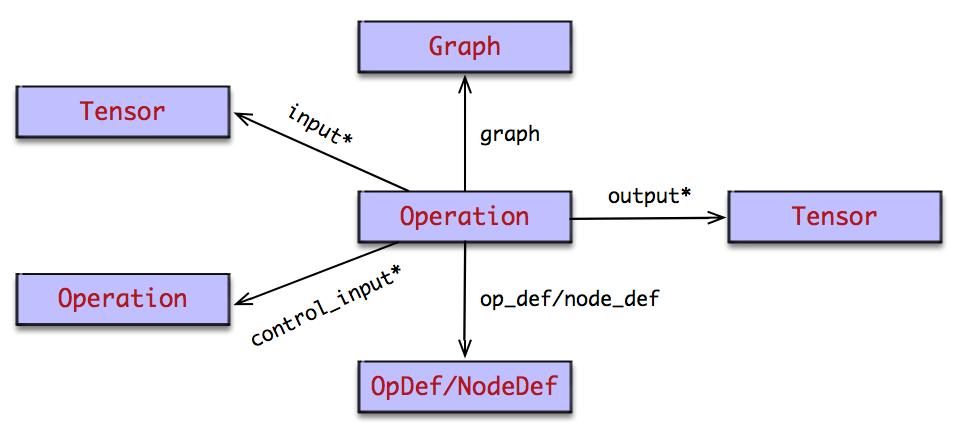
\includegraphics[width=0.8\textwidth]{figures/py-operation.png}
\caption{领域对象:Operation}
 \label{fig:py-operation}
\end{figure}

\subsubsection{构造器}

\begin{leftbar}
\begin{python}
class Operation(object):
  def __init__(self, node_def, g, inputs=None, output_types=None,
               control_inputs=None, input_types=None, original_op=None,
               op_def=None):
    # 1. NodeDef
    self._node_def = copy.deepcopy(node_def)
    
    # 2. OpDef
    self._op_def = op_def

    # 3. Graph
    self._graph = g

    # 4. Input types
    if input_types is None:
      input_types = [i.dtype.base_dtype for i in self._inputs]
    self._input_types = input_types

    # 5. Output types
    if output_types is None:
      output_types = []
    self._output_types = output_types
    
    # 6. Inputs
    if inputs is None:
      inputs = []
    self._inputs = list(inputs)

    # 7. Control Inputs.
    if control_inputs is None:
      control_inputs = []
    
    self._control_inputs = []
    for c in control_inputs:
      c_op = self._get_op_from(c)
      self._control_inputs.append(c_op)

    # 8. Outputs
    self._outputs = [Tensor(self, i, output_type)
                     for i, output_type in enumerate(output_types)]

    # 9. Build producter-consumer relation.
    for a in self._inputs:
      a._add_consumer(self)

    # 10. Allocate unique id for opeartion in graph.
    self._id_value = self._graph._next_id()
\end{python}
\end{leftbar}

\subsubsection{属性集}

\code{Operation}定义了常用了属性方法,用于获取该\ascii{OP}的元数据。其中,\code{name}表示图中节点的名称,包括\code{name\_scope}的层次名称,在图实例的范围内是唯一的,例如\code{relu/MatMul};\code{type}则表示该\code{OP}类型唯一的名称,例如\code{MatMul, Variable}。

\begin{leftbar}
\begin{python}
class Operation(object):
  @property
  def name(self):
    """The full name of this operation."""
    return self._node_def.name

  @property
  def type(self):
    """The type of the op (e.g. `"MatMul"`)."""
    return self._node_def.op

  @property
  def graph(self):
    """The `Graph` that contains this operation."""
    return self._graph

  @property
  def node_def(self):
    """Returns the `NodeDef` proto that represents this operation."""
    return self._node_def

  @property
  def op_def(self):
    """Returns the `OpDef` proto that represents the type of this op."""
    return self._op_def

  @property
  def device(self):
    """The name of the device to which this op has been assigned."""
    return self._node_def.device    
\end{python}
\end{leftbar}

\subsubsection{运行OP}

可以从该\ascii{OP}为末端反向遍历图,寻找最小依赖的子图,并在默认的\code{Session}中执行该子图。

\begin{leftbar}
\begin{python}
class Operation(object):
  def run(self, feed_dict=None, session=None):
    """Runs this operation in a `Session`.

    Calling this method will execute all preceding operations that
    produce the inputs needed for this operation.
    """
    _run_using_default_session(self, feed_dict, session)
\end{python}
\end{leftbar}

其中,\code{\_run\_using\_default\_session}将使用默认的\code{Session}运行该\ascii{OP}。

\begin{leftbar}
\begin{python}
def _run_using_default_session(operation, feed_dict, session=None):
  """Uses the default session to run "operation".
  """
  if session is None:
    session = get_default_session()
  session.run(operation, feed_dict)
\end{python}
\end{leftbar}

\subsection{Tensor}

在图构造期,\code{Tensor}在图中并未承载数据,它仅表示\code{Operation}输出的一个符号句柄。事实上,需要通过\code{Session.run}计算才能得到\code{Tensor}所持有的真实数据。

\subsubsection{生产者与消费者}

如\refig{py-tensor-producter-consumer}所示,\code{Tensor}是两个\code{Operation}数据交换的桥梁,它们之间构造了典型的\emph{生产者与消费者}之间的关系。上游\code{Operation}作为生产者,经过某种抽象计算,生产了一个\code{Tensor},并以此作为该上游\code{Operation}的输出之一,并使用\code{output\_index}作为标识。该\code{Tensor}被传递给下游\code{Operation},并作为下游\code{Operation}的输入,下游\code{Operation}充当该\code{Tensor}的消费者。

\begin{figure}[H]
\centering
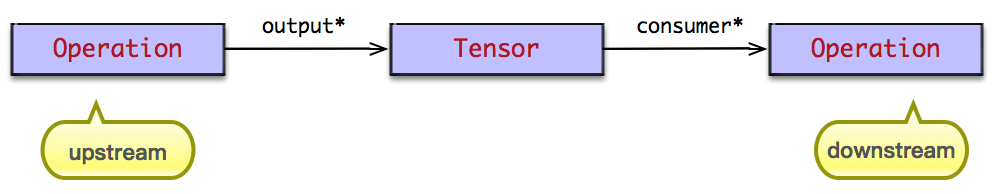
\includegraphics[width=0.8\textwidth]{figures/py-tensor-producter-consumer.png}
\caption{Tensor: 生产者-消费者}
 \label{fig:py-tensor-producter-consumer}
\end{figure}

\subsubsection{领域模型}

如\refig{py-tensor}所示,\code{Tensor}通过\ascii{op}持有扮演生产者角色的\code{Operation},并且使用\code{index}表示该\code{Tensor}在该\code{Operation}输出列表中的索引。也就是说,可以使用\code{op:index}的二元组信息在图中唯一标识一个\code{Tensor}实例。

此外,\code{Tensor}持有\code{Operation}的消费者列表,用于追踪该\code{Tensor}输出到哪些\code{Operation}实例了。因此,\code{Tensor}充当了计算图的边,构建了\code{Operation}之间的数据依赖关系。

\begin{figure}[H]
\centering
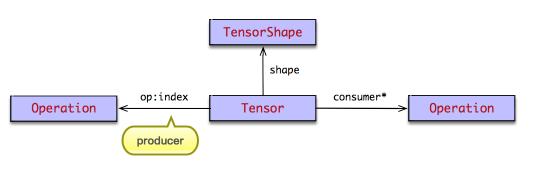
\includegraphics[width=0.9\textwidth]{figures/py-tensor.png}
\caption{领域对象:Tensor}
 \label{fig:py-tensor}
\end{figure}

\subsubsection{建立关联}

最后,参考\code{Operation}与\code{Tensor}的部分实现,很容易找两者之间生产者-消费者的关联关系。当\code{Tensor}列表作为输入流入\code{Operation}时,此时建立了下游\code{Operation}与输入的\code{Tensor}列表之间的消费关系。

\begin{leftbar}
\begin{python}
class Operation(object):
  def __init__(self, node_def, graph, inputs=None, output_types=None):
    # self(Operation) as consumer for input tensors.
    self._inputs = list(inputs)
    for a in self._inputs:
      a._add_consumer(self)

    # self(Operation) as producer for output tensors.
    self._output_types = output_types
    self._outputs = [Tensor(self, i, output_type)
                     for i, output_type in enumerate(output_types)]
\end{python}
\end{leftbar}

同样地,\code{Tensor}在构造器中持有上游的的生产者\code{Operation},及其该\code{Tensor}实例在该\code{Operation}的\code{outputs}列表中的索引。此外,当调用\code{\_add\_consumer},将该下游\code{Operation}追加至消费者列表之中。

\begin{leftbar}
\begin{python}
class Tensor(_TensorLike):
  def __init__(self, op, value_index, dtype):    
    # Index of the OP's endpoint that produces this tensor.
    self._op = op
    self._value_index = value_index
    
    # List of operations that use this Tensor as input.  
    # We maintain this list to easily navigate a computation graph.
    self._consumers = []

  def _add_consumer(self, consumer):
    if not isinstance(consumer, Operation):
      raise TypeError("Consumer must be an Operation: %s" % consumer)
    self._consumers.append(consumer)
\end{python}
\end{leftbar}

\subsubsection{属性集}

通过\code{Tensor}可以追溯上游的\code{Operation},从而获取相关的元数据。可以推测,遍历计算图的算法是反向的,与拓扑排序算法的遍历方向刚好相反。其中,\code{name}返回了\code{(node:output\_index)}的二元组信息,在计算图的范围内唯一地标识了该\code{Tensor}实例。

\begin{leftbar}
\begin{python}
class Tensor(_TensorLike):
  @property
  def op(self):
    """The `Operation` that produces this tensor as an output."""
    return self._op

  @property
  def dtype(self):
    """The `DType` of elements in this tensor."""
    return self._dtype

  @property
  def graph(self):
    """The `Graph` that contains this tensor."""
    return self._op.graph

  @property
  def name(self):
    """The string name of this tensor."""
    return "%s:%d" % (self._op.name, self._value_index)

  @property
  def device(self):
    """The name of the device on which this tensor will be produced."""
    return self._op.device

  @property
  def shape(self):
    """Returns the `TensorShape` that represents the shape of this tensor.
    """
    return self._shape

  @property
  def value_index(self):
    """The index of this tensor in the outputs of its `Operation`."""
    return self._value_index
\end{python}
\end{leftbar}

\subsubsection{评估}

\begin{leftbar}
\begin{python}
class Tensor(_TensorLike):
  def eval(self, feed_dict=None, session=None):
    """Evaluates this tensor in a `Session`.

    Calling this method will execute all preceding operations that
    produce the inputs needed for the operation that produces this
    tensor.
    """
    return _eval_using_default_session(self, feed_dict, self.graph, session)
\end{python}
\end{leftbar}

其中,\code{\_eval\_using\_default\_session}将使用默认的\code{Session}评估该\ascii{Tensor}实例。注意,\code{tf.Session.run}的\code{fetches}列表可以混合接收\code{Operation, Tensor}实例。

\begin{leftbar}
\begin{python}
def _eval_using_default_session(tensors, feed_dict, graph, session=None):
  """Uses the default session to evaluate one or more tensors."""
  if session is None:
    session = get_default_session()
  return session.run(tensors, feed_dict)
\end{python}
\end{leftbar}

\subsection{TensorShape}

\code{Tensor}使用\code{TensorShape}描述其形状信息。它持有该\code{Tensor}的数据类型,及其\code{Dimension}列表,每个\code{Dimension}描述了该维度的大小。其中,\code{TensorShape}与\code{Dimension}都是值对象,包含了一些实用的数学计算方法,例如计数,合并,兼容性检查等。

\begin{figure}[H]
\centering
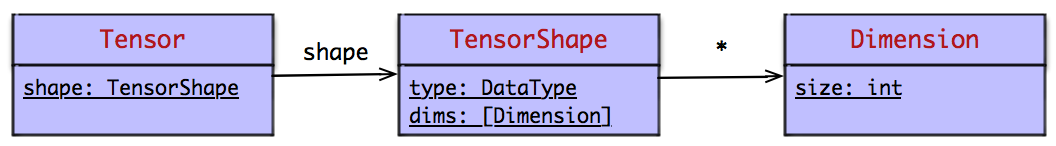
\includegraphics[width=0.9\textwidth]{figures/py-tensor-shape.png}
\caption{TensorShape}
 \label{fig:py-tensor-shape}
\end{figure}

显而易见,可以使用\code{TensorShape}推算出\code{Tensor}所包含的元素个数。

\begin{leftbar}
\begin{python}
class TensorShape(object):
  def num_elements(self):
    if self.is_fully_defined():
      size = 1
      for dim in self._dims:
        size *= dim.value
      return size
    else:
      return None
\end{python}
\end{leftbar}      

\subsubsection{工厂方法}

存在几个实用的工厂方法,\code{scalar, vector, matrix}用于分别构造\ascii{0}维,\ascii{1}维,\ascii{2}维的\code{TensorShape}实例。

\begin{leftbar}
\begin{python}
def scalar():
  return TensorShape([])

def vector(length):
  return TensorShape([length])

def matrix(rows, cols):
  return TensorShape([rows, cols])
\end{python}
\end{leftbar}

\subsubsection{部分定义}

当构造计算图时,对其\code{TensorShape}暂时不能确定,则可以使用\code{None}表示。存在两种情况,如果\code{rank}大小未知,称该\code{TensorShape}未知;如果\code{rank}大小已知,则称该\code{TensorShape}\emph{部分定义}。

\begin{leftbar}
\begin{python}
def unknown_shape(ndims=None):
  if ndims is None:
    return TensorShape(None)
  else:
    return TensorShape([Dimension(None)] * ndims)
\end{python}
\end{leftbar}

\subsubsection{完全定义}

相反地,当\code{TensorShape}每个维度的大小都已确定,则称\emph{完全定义}。

\begin{leftbar}
\begin{python}
class TensorShape(object):
  def is_fully_defined(self):
    return (self._dims is not None and all(dim.value is not None
                                           for dim in self._dims))
\end{python}
\end{leftbar}

\subsubsection{属性集}

可以使用\code{ndims}属性返回\code{TensorShape}的\code{rank}大小,使用\code{dims}属性返回\code{Dimension}列表。

\begin{leftbar}
\begin{python}
class TensorShape(object):
  @property
  def dims(self):
    return self._dims

  @property
  def ndims(self):
    if self._dims is None:
      return None
    else:
      return len(self._dims)
\end{python}
\end{leftbar}

\subsubsection{转换}

可以使用\code{as\_proto}将其转换为\code{TensorShapeProto}表示。特殊地,当某一个\code{Dimension}未知,为了能够实施序列化,需要将\code{None}转换为\ascii{-1}。

\begin{leftbar}
\begin{python} 
class TensorShape(object):
  def _dims_as_proto(self): 
    def _size(dim):
      return -1 if dim.value is None else dim.value
    
    return [tensor_shape_pb2.TensorShapeProto.Dim(size=_size(d))
            for d in self._dims]

  def as_proto(self):
    if self._dims is None:
      return tensor_shape_pb2.TensorShapeProto(unknown_rank=True)
    else:
      return tensor_shape_pb2.TensorShapeProto(dim=self._dims_as_proto())
\end{python}
\end{leftbar}

也可以使用\code{as\_list}将其转为\code{Dimension}列表。如果\code{TensorShape}的\code{rank}大小未知,则抛出\code{ValueError}异常。

\begin{leftbar}
\begin{python} 
class TensorShape(object):
  def as_list(self):
    if self._dims is None:
      raise ValueError("as_list() is not defined on an unknown TensorShape.")
    return [dim.value for dim in self._dims]
\end{python}
\end{leftbar}

相反地,使用\code{as\_shape}将\code{Deimension}列表,或\code{TensorShapeProto}转换为了\code{TensorShape}实例。

\begin{leftbar}
\begin{python}
def as_shape(shape):
  if isinstance(shape, TensorShape):
    return shape
  else:
    return TensorShape(shape)
\end{python}
\end{leftbar}

特殊地,当构造\code{TensorShape}时,当\code{TensorShapeProto}的某一维度大小为\ascii{-1}时,将其转换为\code{None}的表示。

\begin{leftbar}
\begin{python}
class TensorShape(object):
  def __init__(self, dims):
    if dims is None:
      self._dims = None
    elif isinstance(dims, tensor_shape_pb2.TensorShapeProto):
      if dims.unknown_rank:
        self._dims = None
      else:
        self._dims = [
          as_dimension(dim.size if dim.size != -1 else None)
          for dim in dims.dim
        ]
    elif isinstance(dims, TensorShape):
      self._dims = dims.dims
    else:
      try:
        dims_iter = iter(dims)
      except TypeError:
        # Treat as a singleton dimension
        self._dims = [as_dimension(dims)]
      else:
        # Got a list of dimensions
        self._dims = [as_dimension(d) for d in dims_iter]
\end{python}
\end{leftbar}

\subsection{Graph}

\code{Graph}是\tf{}最重要的领域对象,\tf{}的运行时就是完成\code{Graph}的构造、传递、剪枝、优化、分裂、执行。因此,熟悉\code{Graph}的领域模型,对于理解整个\tf{}运行时大有裨益。

\subsubsection{领域模型}

如\refig{py-graph}所示,一个\code{Graph}对象将包含一系列\code{Operation}对象,表示计算单元的集合。同时,它间接持有一系列\code{Tensor}对象,表示数据单元的集合。

\begin{figure}[H]
\centering
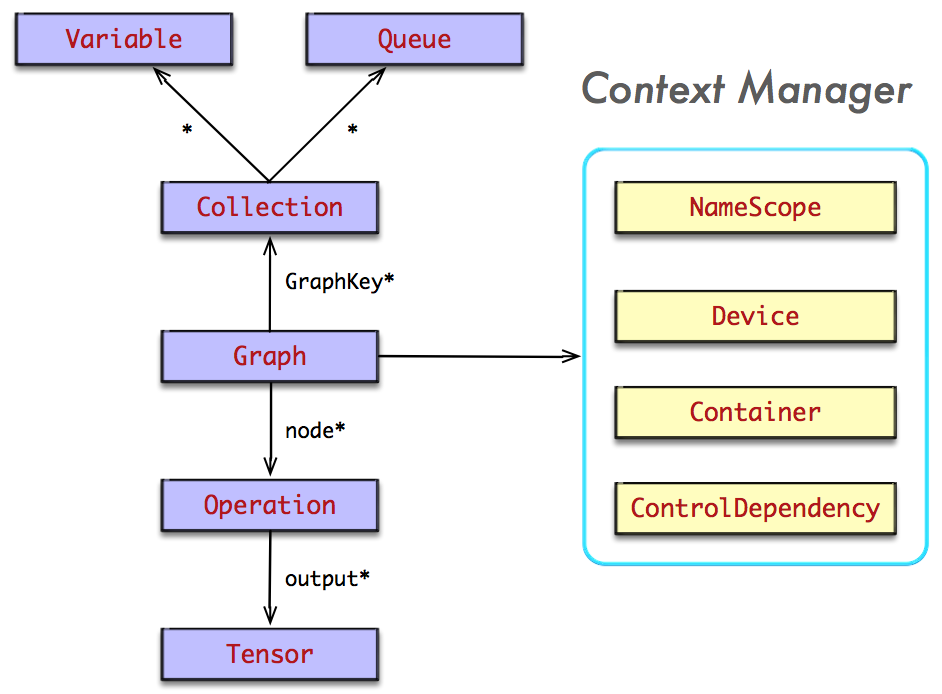
\includegraphics[width=0.8\textwidth]{figures/py-graph.png}
\caption{领域对象:Graph}
 \label{fig:py-graph}
\end{figure}

为了快速索引图中的节点信息,在当前图的作用域内为每个\code{Operation}分配唯一的\code{id},并在图中存储\code{\_nodes\_by\_id}的数据字典。同时,为了可以根据节点的名字快速索引节点信息,在图中也存储了\code{\_nodes\_by\_name}的数据字典。

\begin{leftbar}
\begin{python}
class Graph(object):
  def __init__(self):
    self._lock = threading.Lock()
    self._nodes_by_id = dict()    # GUARDED\_BY(self.\_lock)
    self._next_id_counter = 0     # GUARDED\_BY(self.\_lock)
    self._nodes_by_name = dict()  # GUARDED\_BY(self.\_lock)
    self._version = 0             # GUARDED\_BY(self.\_lock)
\end{python}
\end{leftbar}

在图构造期,\code{OP}通过\ascii{OP}构造器创建,最终被添加至当前的\code{Graph}实例中。当图被冻结后,便不能往图中追加节点了,使得\code{Graph}实例在多线程中被安全地共享。

\begin{leftbar}
\begin{python}
class Graph(object):
  def _add_op(self, op):
    self._check_not_finalized()
    with self._lock:
      self._nodes_by_id[op._id] = op
      self._nodes_by_name[op.name] = op
      self._version = max(self._version, op._id)
\end{python}
\end{leftbar}

\subsubsection{分组}

为了更好地管理\code{Graph}中的节点,在每个\code{Operation}上打上特定的标签,实现了节点的分类。相同类型的节点被划归在同一个\code{Collection}中,并使用唯一的\code{GraphKey}标识该集合。随后,便可以根据\code{GraphKey}快速索引相关的节点信息。其中,系统预定义了常用的\code{GraphKey},同时也支持自定义的\code{GraphKey}。

\begin{leftbar}
\begin{python}
class GraphKeys(object):
  # Key to collect Variable objects that are global (shared across machines).
  # Default collection for all variables, except local ones.
  GLOBAL_VARIABLES = "variables"

  # Key to collect local variables that are local to the machine and are not
  # saved/restored.
  LOCAL_VARIABLES = "local_variables"

  # Key to collect model variables defined by layers.
  MODEL_VARIABLES = "model_variables"

  # Key to collect Variable objects that will be trained by the
  # optimizers.
  TRAINABLE_VARIABLES = "trainable_variables"

  # Key to collect summaries.
  SUMMARIES = "summaries"

  # Key to collect QueueRunners.
  QUEUE_RUNNERS = "queue_runners"

  # Key to collect table initializers.
  TABLE_INITIALIZERS = "table_initializer"

  # Key to collect asset filepaths. An asset represents an external resource
  # like a vocabulary file.
  ASSET_FILEPATHS = "asset_filepaths"

  # Key to collect Variable objects that keep moving averages.
  MOVING_AVERAGE_VARIABLES = "moving_average_variables"
  # Key to collect regularization losses at graph construction.

  REGULARIZATION_LOSSES = "regularization_losses"

  # Key to collect concatenated sharded variables.
  CONCATENATED_VARIABLES = "concatenated_variables"

  # Key to collect savers.
  SAVERS = "savers"

  # Key to collect weights
  WEIGHTS = "weights"

  # Key to collect biases
  BIASES = "biases"

  # Key to collect activations
  ACTIVATIONS = "activations"

  # Key to collect update\_ops
  UPDATE_OPS = "update_ops"

  # Key to collect losses
  LOSSES = "losses"

  # Key to collect BaseSaverBuilder.SaveableObject instances for checkpointing.
  SAVEABLE_OBJECTS = "saveable_objects"

  # Key to collect all shared resources used by the graph which need to be
  # initialized once per cluster.
  RESOURCES = "resources"

  # Key to collect all shared resources used in this graph which need to be
  # initialized once per session.
  LOCAL_RESOURCES = "local_resources"

  # Trainable resource-style variables.
  TRAINABLE_RESOURCE_VARIABLES = "trainable_resource_variables"

  # Key to indicate various ops.
  INIT_OP = "init_op"
  LOCAL_INIT_OP = "local_init_op"
  READY_OP = "ready_op"
  READY_FOR_LOCAL_INIT_OP = "ready_for_local_init_op"
  SUMMARY_OP = "summary_op"
  GLOBAL_STEP = "global_step"

  # Used to count the number of evaluations performed during a 
  # single evaluation run.
  EVAL_STEP = "eval_step"
  TRAIN_OP = "train_op"

  # Key for control flow context.
  COND_CONTEXT = "cond_context"
  WHILE_CONTEXT = "while_context"
\end{python}
\end{leftbar}

当某个\code{Opeartion}创建时,可以将其划归在特定的集合中,便于后期根据\code{GraphKey}快速索引。

\begin{leftbar}
\begin{python}
class Graph(object):
  def add_to_collection(self, name, value):
    self._check_not_finalized()
    with self._lock:
      if name not in self._collections:
        self._collections[name] = [value]
      else:
        self._collections[name].append(value)
\end{python}
\end{leftbar}


\subsubsection{图实例}

一般地,\ascii{OP}注册到一个全局的、唯一的、隐式的、默认的图实例中。特殊地,\tf{}也可以显式地创建新的图实例\code{g},并调用\code{g.as\_default()}使其成为当前线程中唯一默认的图实例,并在该上下文管理器中所创建的\ascii{OP}都将自动注册到该图实例中。

\begin{leftbar}
\begin{python}
with tf.Graph().as_default() as g:
  c = tf.constant(5.0)
  assert c.graph is g
\end{python}
\end{leftbar}

事实上,\code{g.as\_default}从当前线程的图栈中返回了一个上下文管理器,使得当前的图实例\code{g}覆盖原来默认的图实例;当退出了上下文管理器后,则恢复原来默认的图实例。但是,在任何一个时刻,在当前线程中有且仅有一个图实例成为\emph{默认的},可以调用\code{tf.get\_default\_graph()},返回该默认的图实例。

\begin{leftbar}
\begin{python}
_default_graph_stack = _DefaultGraphStack()

def get_default_graph():
  """Returns the default graph for the current thread."""
  return _default_graph_stack.get_default()

class Graph(object):
  def as_default(self):
    """Returns a context manager that makes this `Graph` the default graph."""
    return _default_graph_stack.get_controller(self)
\end{python}
\end{leftbar}

其中,\code{\_DefaultStack}中的\code{get\_controller}在栈顶追加新的图实例;当退出上下文管理器后,则从栈顶移除该图实例,恢复之前的图实例。当调用\code{get\_default}时,如果栈为空则通过\code{\_GetGlobalDefaultGraph}返回全局的、唯一的、隐式的图实例。在大部分\tf{}程序中,如果没有显式创建多个图实例,则所有\ascii{OP}都默认地注册到该图实例中。

\begin{leftbar}
\begin{python}
class _DefaultStack(threading.local):
  """A thread-local stack for providing implicit defaults."""

  def __init__(self):
    super(_DefaultStack, self).__init__()
    self.stack = []

  def get_default(self):
    return self.stack[-1] if len(self.stack) >= 1 else None

  @tf_contextlib.contextmanager
  def get_controller(self, default):
    """A context manager for manipulating a default stack."""
    try:
      self.stack.append(default)
      yield default
    finally:
      self.stack.remove(default)

class _DefaultGraphStack(_DefaultStack):
  """A thread-local stack for providing an implicit default graph."""

  def __init__(self):
    super(_DefaultGraphStack, self).__init__()
    self._global_default_graph = None

  def get_default(self):
    """Override that returns a global default if the stack is empty."""
    ret = super(_DefaultGraphStack, self).get_default()
    if ret is None:
      ret = self._GetGlobalDefaultGraph()
    return ret

  def _GetGlobalDefaultGraph(self):
    if self._global_default_graph is None:
      self._global_default_graph = Graph()
    return self._global_default_graph
\end{python}
\end{leftbar}

\subsubsection{名字空间}

为了更好地管理图中的节点,使用\code{name\_scope}对图中的节点实施层次化命名。例如,想要在全宇宙的范围内定位故宫的位置,可以实施层次化的命名:宇宙/银河系/太阳系/地球/中国/北京/故宫。这对于\ascii{TensorBoard}实现计算图的可视化非常有帮助,当计算图比较大时,可以通过折叠的方式展示图,也可以通过展开的方式一窥究竟。

内嵌的\code{name\_scope}将继承外围的\code{name\_scope};如果内嵌的\code{name\_scope}以\code{/}结尾,将重置为指定的\code{name\_scope};如果内嵌的\code{name\_scope}为空字符串或\code{None},将重置整个\code{name\_scope}。

\begin{leftbar}
\begin{python}
with tf.Graph().as_default() as g:
  with g.name_scope("nested") as scope:
    nested_c = tf.constant(10.0, name="c")
    assert nested_c.op.name == "nested/c"

    # Create a nested scope called "inner".
    with g.name_scope("inner"):
      nested_inner_c = tf.constant(30.0, name="c")
      assert nested_inner_c.op.name == "nested/inner/c"

      # Treats `scope` as an absolute name scope, 
      # and switches to the "nested/" scope.
      with g.name_scope(scope):
        nested_d = tf.constant(40.0, name="d")
        assert nested_d.op.name == "nested/d"

        # reset name scope
        with g.name_scope(""):
          e = tf.constant(50.0, name="e")
          assert e.op.name == "e"
\end{python}
\end{leftbar}

事实上,\code{name\_scope}是一个上下文管理器,在嵌套的\code{name\_scope}中,实现了\code{name\_scope}栈式管理。当\code{name\_scope}出了作用域,便自动恢复外围的\code{name\_scope}。

\begin{leftbar}
\begin{python}
def _name_from_scope_name(name):
  return name[:-1] if name[-1] == "/" else name

class Graph(object):
  def __init__(self):
    self._name_stack = ""

  @tf_contextlib.contextmanager
  def name_scope(self, name):
    try:
      old_stack = self._name_stack
      if not name:
        new_stack = None
      elif name and name[-1] == "/":
        new_stack = _name_from_scope_name(name)
      else:
        new_stack = self.unique_name(name)
      self._name_stack = new_stack
      yield "" if new_stack is None else new_stack + "/"
    finally:
      self._name_stack = old_stack
\end{python}
\end{leftbar}

在图构造期,\ascii{OP}构造器更习惯于使用\code{tf.name\_scope},它从输入的\code{Operation}或\code{Tensor}列表中尝试获取图实例;如果未能获取到,则返回默认的图实例。然后,再在该图实例上追加新的\code{name\_scope}。

\begin{leftbar}
\begin{python}
@tf_contextlib.contextmanager
def name_scope(name, default_name=None, values=[]):
  n = default_name if name is None else name
  g = _get_graph_from_inputs(values)
  with g.as_default(), g.name_scope(n) as scope:
    yield scope
\end{python}
\end{leftbar}

\subsubsection{控制依赖}

可以通过内嵌的\code{control\_dependencies}合并外围的\code{control\_dependencies},或通过\code{None}重置控制依赖集合为空。

\begin{leftbar}
\begin{python}
with g.control_dependencies([a, b]):
  # Ops constructed here run after `a` and `b`.
  with g.control_dependencies(None):
    # Ops constructed here not waiting for either `a` or `b`.
    with g.control_dependencies([c, d]):
      # Ops constructed here run after `c` and `d`, 
      # also not waiting for either `a` or `b`.
  with g.control_dependencies([e, f]):
    # Ops constructed here run after `a, b, e, f`.
\end{python}
\end{leftbar}

事实上,\code{control\_dependencies}返回了一个上下文管理器,用于指定\ascii{OP}的控制依赖关系。其中,\code{control\_ops}记录了当前层所依赖的\ascii{Operation}列表,而\code{current}记录了当前层,及其外围所依赖的所有\ascii{Operation}列表。

\begin{leftbar}
\begin{python}
class Graph(object):
  def control_dependencies(self, control_inputs):
    if control_inputs is None:
      return self._ControlDependenciesController(self, None)

    control_ops = []
    current = self._current_control_dependencies()
    for c in control_inputs:
      c = self.as_graph_element(c)
      if isinstance(c, Tensor):
        c = c.op
      if c not in current:
        control_ops.append(c)
        current.add(c)
    return self._ControlDependenciesController(self, control_ops)
\end{python}
\end{leftbar}

\code{\_ControlDependenciesController}实现了一个控制依赖的控制器。\code{control\_inputs}为\code{None},将启用一个新的作用域,从而实现了新栈替代旧栈;当退出当前上下文的作用域后,恢复之前的旧栈,从而清除了所有之前的控制依赖关系。否则,每进入一层\code{control\_inputs},便叠加当前作用域到当前的栈中。

\begin{leftbar}
\begin{python}
class Graph(object):
  def __init__(self):
    self._control_dependencies_stack = []

  def _push_control_dependencies_controller(self, controller):
    self._control_dependencies_stack.append(controller)

  def _pop_control_dependencies_controller(self):
    self._control_dependencies_stack.pop()

  class _ControlDependenciesController(object):
    """Context manager for `control\_dependencies()`."""

    def __init__(self, graph, control_inputs):
      self._graph = graph
      if control_inputs is None:
        self._control_inputs = []
        self._new_stack = True
      else:
        self._control_inputs = control_inputs
        self._new_stack = False
      self._seen_nodes = set()
      self._old_stack = None

    def __enter__(self):
      if self._new_stack:
        # Clear the control\_dependencies.
        self._old_stack = self._graph._control_dependencies_stack
        self._graph._control_dependencies_stack = []
      self._graph._push_control_dependencies_controller(self)

    def __exit__(self, unused_type, unused_value, unused_traceback):
      self._graph._pop_control_dependencies_controller()
      if self._new_stack:
        self._graph._control_dependencies_stack = self._old_stack
\end{python}
\end{leftbar}

\code{\_current\_control\_dependencies}用于规约所有外围的\code{control\_inputs},直至当前层所依赖的\code{Operation}列表。

\begin{leftbar}
\begin{python}
class Graph(object):
  def _current_control_dependencies(self):
    ret = set()
    for controller in self._control_dependencies_stack:
      for op in controller.control_inputs:
        ret.add(op)
    return ret
\end{python}
\end{leftbar}

\subsubsection{容器}

\begin{leftbar}
\begin{python}
with g.container('experiment0'):
  # All stateful Operations constructed in this context will be placed
  # in resource container "experiment0".
  v1 = tf.Variable([1.0])
  v2 = tf.Variable([2.0])
  with g.container("experiment1"):
    # All stateful Operations constructed in this context will be
    # placed in resource container "experiment1".
    v3 = tf.Variable([3.0])
    q1 = tf.FIFOQueue(10, tf.float32)
  # All stateful Operations constructed in this context will be
  # be created in the "experiment0".
  v4 = tf.Variable([4.0])
  q1 = tf.FIFOQueue(20, tf.float32)
  with g.container(""):
    # All stateful Operations constructed in this context will be
    # be placed in the default resource container.
    v5 = tf.Variable([5.0])
    q3 = tf.FIFOQueue(30, tf.float32)

# Resets container "experiment0", after which the state of v1, v2, v4, q1
# will become undefined (such as uninitialized).
tf.Session.reset(target, ["experiment0"])
\end{python}
\end{leftbar}

\begin{leftbar}
\begin{python}
class Graph(object):
  @tf_contextlib.contextmanager
  def container(self, container_name):
    """Returns a context manager that specifies the resource container."""
    original_container = self._container
    try:
      self._container = container_name
      yield self._container
    finally:
      self._container = original_container
\end{python}
\end{leftbar}

\subsection{图构造}

在计算图的构造期间,不执行任何\ascii{OP}的计算。简单地说,图的构造过程就是根据\ascii{OP}构造器完成\code{Operation}实例的构造。而在\code{Operation}实例的构造之前,需要实现完成\code{OpDef}与\code{NodeDef}的构造过程。

\subsubsection{OpDef仓库}

\code{OpDef}仓库在系统首次访问时,实现了\code{OpDef}的延迟加载和注册。也就是说,对于某中类型的\code{OpDef}仓库,\code{\_InitOpDefLibrary}模块首次导入时,扫描\code{op\_list\_ascii}表示的所有\ascii{OP},并将其转换为\ascii{Protobuf}格式的\code{OpList}实例,最终将其注册到\code{OpDefLibrary}实例之中。

例如,模块\code{gen\_array\_ops}是构建版本时自动生成的,它主要完成所有\code{array\_ops}类型的\code{OpDef}的定义,并自动注册到\code{OpDefLibrary}的仓库实例中,并提供按名查找\code{OpDef}的服务接口。

\begin{leftbar}
\begin{python}
_op_def_lib = _InitOpDefLibrary()

def _InitOpDefLibrary():
  op_list = _op_def_pb2.OpList()
  _text_format.Merge(_InitOpDefLibrary.op_list_ascii, op_list)   
  op_def_lib = _op_def_library.OpDefLibrary()
  op_def_lib.add_op_list(op_list)
  return op_def_lib

_InitOpDefLibrary.op_list_ascii = """op {
  name: "ZerosLike"
  input_arg {
    name: "x"
    type_attr: "T"
  }
  output_arg {
    name: "y"
    type_attr: "T"
  }
  attr {
    name: "T"
    type: "type"
  }
}
# ignore others
"""
\end{python}
\end{leftbar}

\subsubsection{工厂方法}

如\refig{py-op-factory-and-repo}所示。当\ascii{Client}使用\ascii{OP}构造器创建一个\code{Operation}实例时,将最终调用\code{Graph.create\_op}方法,将该\code{Operation}实例注册到该图实例中。

也就是说,一方面,\code{Graph}充当\code{Operation}的工厂,负责\code{Operation}的创建职责;另一方面,\code{Graph}充当\code{Operation}的仓库,负责\code{Operation}的存储,检索,转换等操作。

这个过程常称为计算图的构造。在计算图的构造期间,并不会触发运行时的\ascii{OP}运算,它仅仅描述计算节点之间的依赖关系,并构建\ascii{DAG}图,对整个计算过程做整体规划。

\begin{figure}[!htbp]
\centering
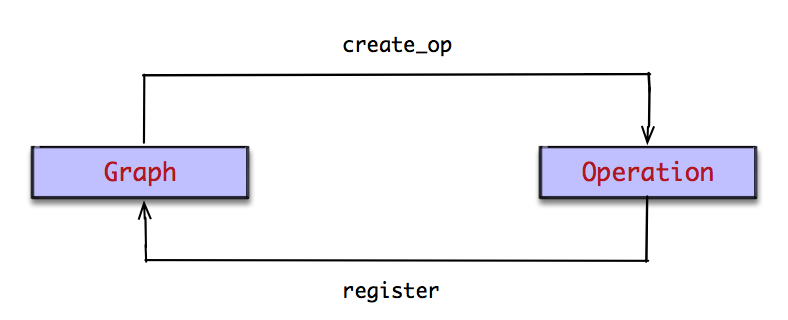
\includegraphics[width=0.9\textwidth]{figures/py-op-factory-and-repo.png}
\caption{Graph: OP工厂 + OP仓库}
 \label{fig:py-op-factory-and-repo}
\end{figure}

\subsubsection{OP构造器}

如\refig{py-op-constructor}所示。在图构造期,\ascii{Client}使用\code{tf.zeros\_like}构造一个名为\code{ZerosLike}的\ascii{OP},该\ascii{OP}拥有一个输入,输出一个全\ascii{0}的\ascii{Tensor};其中,\code{tf.zeros\_like}常称为\ascii{OP}构造器。

然后,\ascii{OP}构造器调用一段自动生成的代码,进而转调\code{OpDefLibrary.apply\_op}方法。

\begin{figure}[!htbp]
\centering
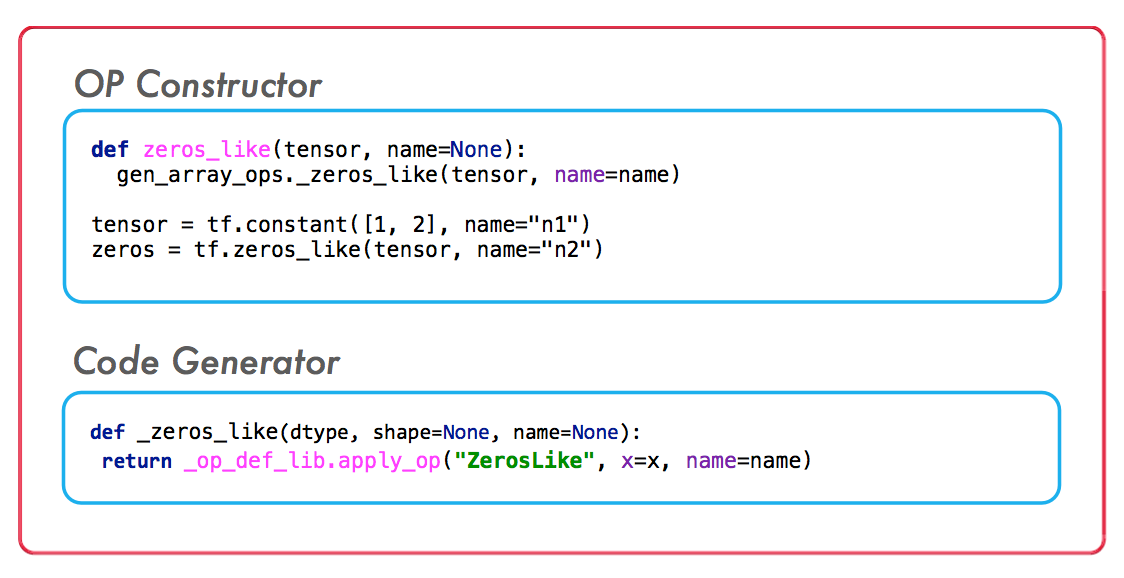
\includegraphics[width=0.9\textwidth]{figures/py-op-constructor.png}
\caption{OP构造器与代码生成器}
 \label{fig:py-op-constructor}
\end{figure}

\subsubsection{构造OpDef与NodeDef}

然后,如\refig{py-graph-create-op}所示。\code{OpDefLibrary}根据\ascii{OP}的名字从\code{OpDefLibrary}中,找到对应\code{OpDef}实例;最终,通过\code{Graph.create\_op}的工厂方法,创建\code{NodeDef}实例,进而创建\code{Operation}实例,将其自身注册到图实例中。

\begin{figure}[!htbp]
\centering
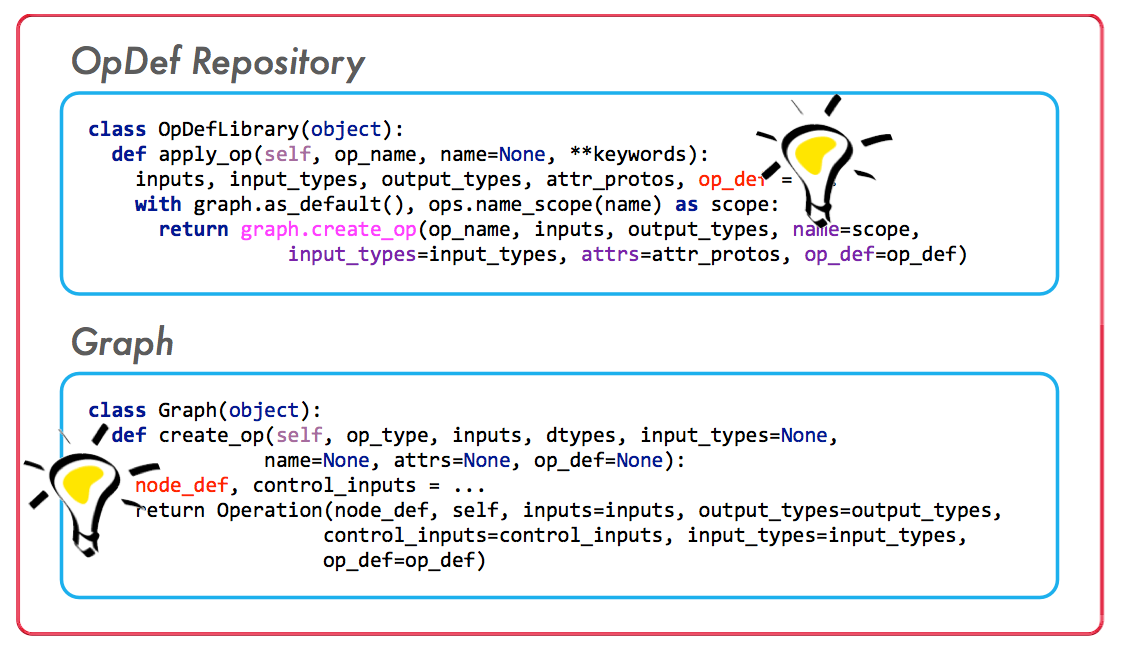
\includegraphics[width=0.9\textwidth]{figures/py-graph-create-op.png}
\caption{创建Operation实例: 创建OpDef, NodeDef实例}
 \label{fig:py-graph-create-op}
\end{figure}

\end{content}

\section{后端C++}

\begin{content}

在\ascii{C++}后端,计算图是\ascii{TensorFlow}领域模型的核心。

\subsection{边}

\code{Edge}持有前驱节点与后驱节点,从而实现了计算图的连接。一个节点可以拥有零条或多条输入边,与可以有零条或多条输出边。一般地,计算图中存在两类边:

\begin{enum}
  \eitem{普通边:用于承载数据(以\code{Tensor}表示),表示节点间“生产者-消费者”的数据依赖关系,常用实线表示;}
  \eitem{控制依赖:不承载数据,用于表示节点间的执行依赖关系,常用虚线表示。} 
\end{enum}

\subsubsection{两个标识}

\ascii{Edge}持有两个重要的索引:

\begin{enum}
  \eitem{\code{src\_output}:表示该边为「前驱节点」的第\code{src\_output}条输出边;}
  \eitem{\code{dst\_input}:表示该边为「后驱节点」的第\code{dst\_input}条输入边。} 
\end{enum}


\begin{figure}[!htbp]
\centering
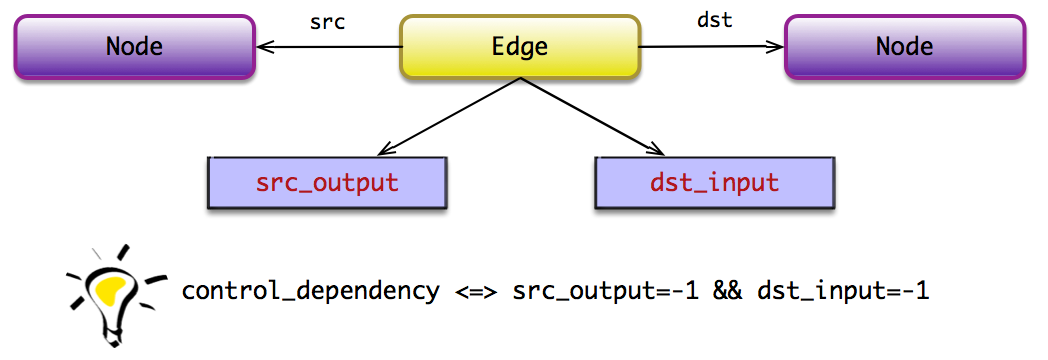
\includegraphics[width=0.9\textwidth]{figures/cc-edge-model.png}
\caption{领域对象:Edge}
 \label{fig:cc-edge-model}
\end{figure}

例如,存在两个前驱节点\code{s1, s2},都存在两条输出边;存在两个后驱节点\code{d1, d2},都存在两条输入边。

\begin{figure}[!htbp]
\centering
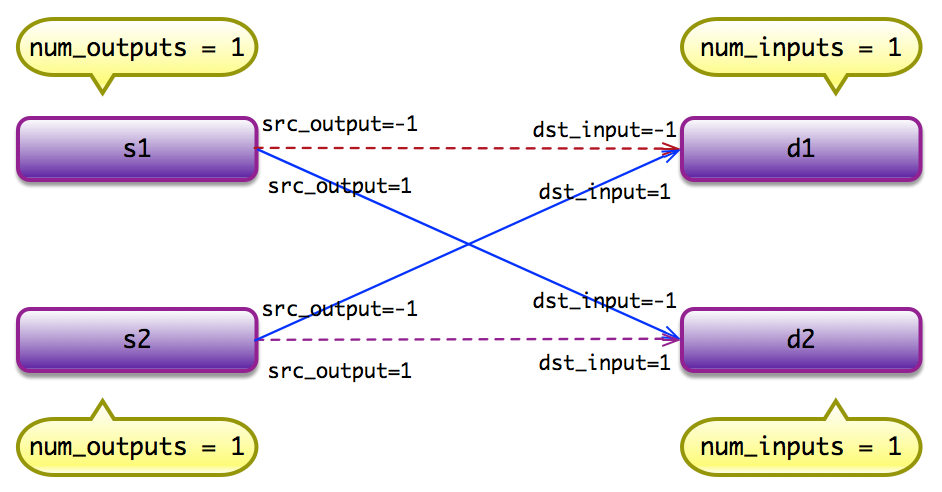
\includegraphics[width=0.9\textwidth]{figures/cc-edge-model-example.png}
\caption{边例子}
 \label{fig:cc-edge-model-example}
\end{figure}

\subsubsection{控制依赖}

对于控制依赖边,其\code{src\_output, dst\_input}都为\code{-1(Graph::kControlSlot)},暗喻控制依赖边不承载任何数据。

\begin{leftbar}
\begin{c++}
bool Edge::IsControlEdge() const {
   // or dst\_input\_ == Graph::kControlSlot;
   return src_output_ == Graph::kControlSlot;
}
\end{c++}
\end{leftbar}

\subsubsection{Tensor标识}

一般地,计算图的「普通边」承载\code{Tensor},并使用\code{TensorId}标识。\code{Tensor}标识由源节点的名字,及其所在边的\code{src\_output}唯一确定。

\begin{leftbar}
\begin{c++}
TensorId ::= node_name:src_output
\end{c++}
\end{leftbar}

缺省地,\code{src\_output}默认为\ascii{0};也就是说,\code{node\_name}与\code{node\_name:0}两者等价。特殊地,当\code{src\_output}等于\ascii{-1}时,表示该边为「控制依赖边」,\code{TensorId}可以标识为\code{\^node\_name},标识该边依赖于\code{node\_name}所在的节点。

\subsection{节点}

\code{Node}(节点)可以拥有零条或多条输入/输出的边,并使用\code{in\_edges, out\_edges}分别表示输入边和输出边的集合。另外,\code{Node}持有\code{NodeDef, OpDef}。其中,\code{NodeDef}包含设备分配信息,及其\ascii{OP}的属性值列表;\code{OpDef}持有\ascii{OP}的元数据,包括\ascii{OP}输入输出类型等信息。

\begin{figure}[!htbp]
\centering
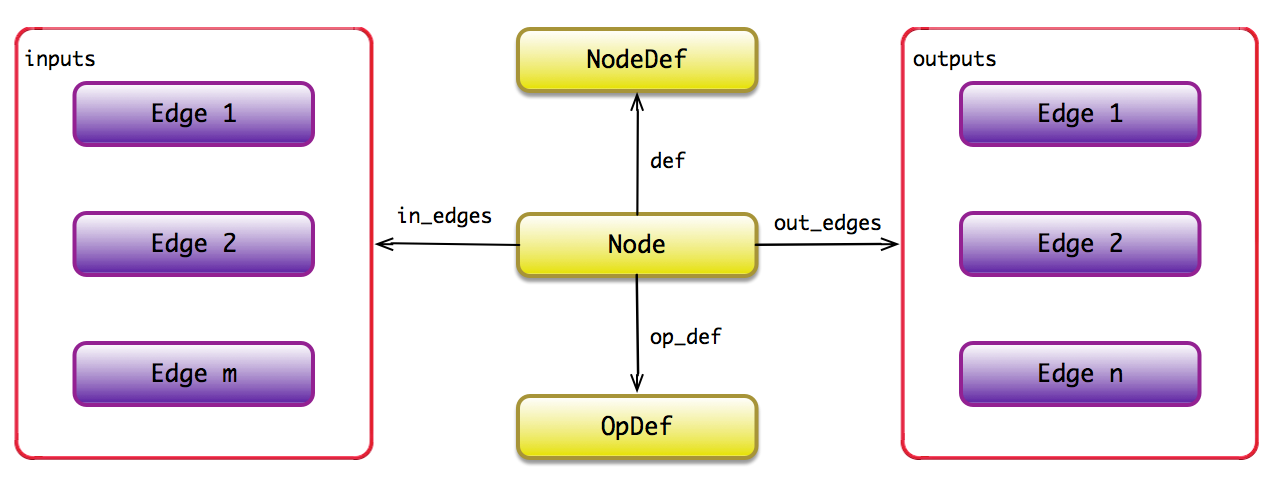
\includegraphics[width=0.9\textwidth]{figures/cc-node-model.png}
\caption{领域对象:Node}
 \label{fig:cc-node-model}
\end{figure}

\subsubsection{输入边}

在输入边的集合中,可以按照索引\code{(dst\_input)}线性查找。当节点输入的边比较多时,可能会成为性能的瓶颈。依次类推,按照索引\code{(src\_output)}查找输出边,算法类同。

\begin{leftbar}
\begin{c++}
Status Node::input_edge(int idx, const Edge** e) const {
  for (auto edge : in_edges()) {
    if (edge->dst_input() == idx) {
      *e = edge;
      return Status::OK();
    }
  }
  return errors::NotFound("not found input edge ", idx);
}
\end{c++}
\end{leftbar}

\subsubsection{前驱节点}

首先通过\code{idx}索引找到输入边,然后通过输入边找到前驱节点。依次类推,按照索引查找后驱节点,算法类同。

\begin{leftbar}
\begin{c++}
Status Node::input_node(int idx, const Node** n) const {
  const Edge* e = nullptr;
  TF_RETURN_IF_ERROR(input_edge(idx, &e));
  *n = e == nullptr ? nullptr : e->src();
  return Status::OK();
}
\end{c++}
\end{leftbar}

\subsection{图}

\code{Graph}(计算图)就是节点与边的集合。计算图是一个\ascii{DAG}图,计算图的执行过程将按照\ascii{DAG}的拓扑排序,依次启动\ascii{OP}的运算。其中,如果存在多个入度为\ascii{0}的节点,\ascii{TensorFlow}运行时可以实现并发,同时执行多个\ascii{OP}的运算,提高执行效率。

\begin{figure}[!htbp]
\centering

\includegraphics[width=0.9\textwidth]{figures/cc-graph-model.png}
\caption{领域模型:图}
 \label{fig:cc-graph-model}
\end{figure}

\subsubsection{空图}

计算图的初始状态,并非是一个空图。实现添加了两个特殊的节点:\code{Source}与\code{Sink}节点,分别表示\ascii{DAG}图的起始节点与终止节点。其中,\code{Source}的\code{id}为\ascii{0},\code{Sink}的\code{id}为\ascii{1};依次论断,普通\ascii{OP}节点的\ascii{id}将大于\ascii{1}。

\code{Source}与\code{Sink}之间,通过连接「控制依赖」的边,保证计算图的执行始于\code{Source}节点,终于\code{Sink}节点。它们之前的控制依赖边,其\code{src\_output, dst\_input}值都为\ascii{-1}。

\begin{figure}[!htbp]
\centering
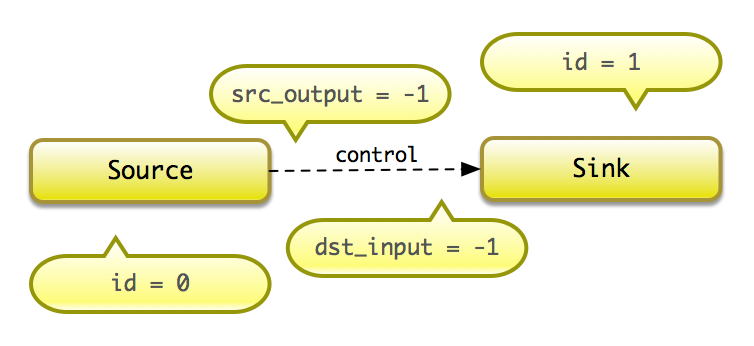
\includegraphics[width=0.9\textwidth]{figures/cc-empty-graph.png}
\caption{空图}
 \label{fig:cc-empty-graph}
\end{figure}

\code{Source}与\code{Sink}是两个内部实现保留的节点,其节点名称以下划线开头,分别使用\code{\_SOURCE}和\code{\_SINK}命名;并且,它们都是\code{NoOp},表示不执行任何计算。

\begin{leftbar}
\begin{c++}
Node* Graph::AddInternalNode(const char* name, int id) {
  NodeDef def;
  def.set_name(name);
  def.set_op("NoOp");

  Status status;
  Node* node = AddNode(def, &status);
  TF_CHECK_OK(status);
  CHECK_EQ(node->id(), id);
  return node;
}

Graph::Graph(const OpRegistryInterface* ops)
    : ops_(ops), arena_(8 << 10 /* 8kB */) {
  auto src  = AddInternalNode("_SOURCE", kSourceId);
  auto sink = AddInternalNode("_SINK",   kSinkId);
  AddControlEdge(src, sink);
}
\end{c++}
\end{leftbar}

习惯上,仅包含\code{Source}与\code{Sink}节点的计算图也常常称为空图。

\subsubsection{非空图}

在前端,用户使用\ascii{OP}构造器,将构造任意复杂度的计算图。对于运行时,实现将用户构造的计算图通过控制依赖的边与\code{Source/Sink}节点连接,保证计算图执行始于\code{Source}节点,终于\code{Sink}节点。

\begin{figure}[!htbp]
\centering
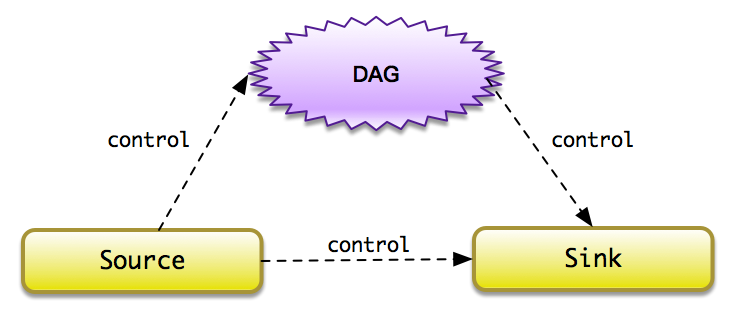
\includegraphics[width=0.9\textwidth]{figures/cc-non-empty-graph.png}
\caption{非空图}
 \label{fig:cc-non-empty-graph}
\end{figure}

\subsubsection{添加边}

计算图的构造过程非常简单,首先通过\code{Graph::AddNode}在图中放置节点,然后再通过\code{Graph::AddEdge}在图中放置边,实现节点之间的连接。

\begin{leftbar}
\begin{c++}
const Edge* Graph::AllocEdge() const {
  Edge* e = nullptr;
  if (free_edges_.empty()) {
    e = new (arena_.Alloc(sizeof(Edge))) Edge;
  } else {
    e = free_edges_.back();
    free_edges_.pop_back();
  }
  e->id_ = edges_.size();
  return e;
}

const Edge* Graph::AddEdge(Node* source, int x, Node* dest, int y) {
  auto e = AllocEdge();
  e->src_ = source;
  e->dst_ = dest;
  e->src_output_ = x;
  e->dst_input_ = y;

  CHECK(source->out_edges_.insert(e).second);
  CHECK(dest->in_edges_.insert(e).second);

  edges_.push_back(e);
  edge_set_.insert(e);
  return e;
}
\end{c++}
\end{leftbar}

\subsubsection{添加控制依赖边}

添加控制依赖边,则可以转发调用\code{Graph::AddEdge}实现;此时,\code{src\_output, dst\_input}都为\ascii{-1}。

\begin{leftbar}
\begin{c++}
const Edge* Graph::AddControlEdge(Node* src, Node* dst) {
  return AddEdge(src, kControlSlot, dst, kControlSlot);
}
\end{c++}
\end{leftbar}

\subsection{OpDef仓库}

同样地,\code{OpDef}仓库在\ascii{C++}系统\code{main}函数启动之前完成\code{OpDef}的加载和注册。它使用\ascii{REGISTER\_OP}宏完成\ascii{OpDef}的注册。

\begin{figure}[!htbp]
\centering
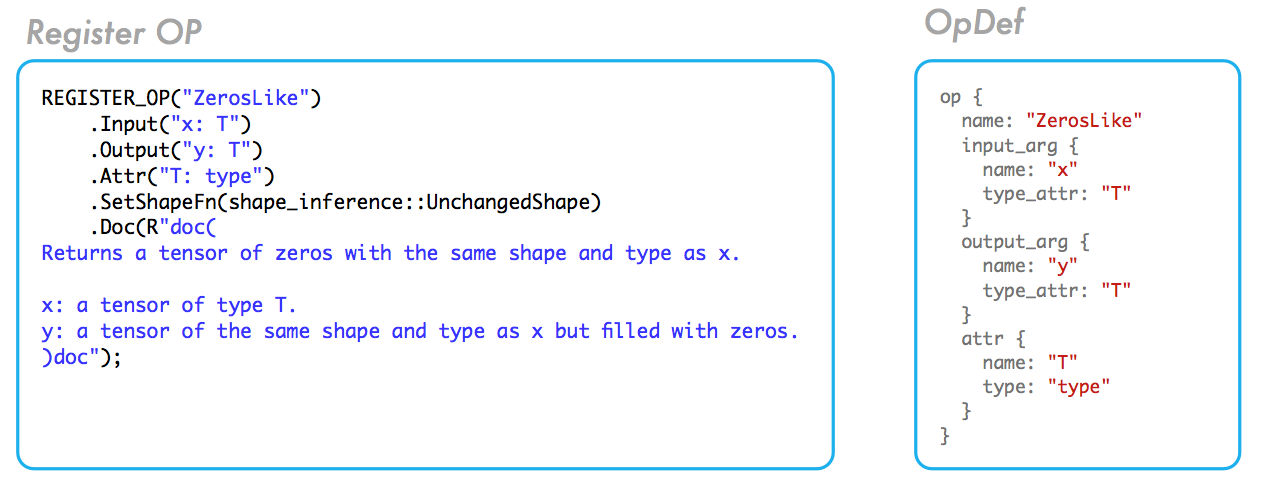
\includegraphics[width=0.9\textwidth]{figures/cc-op-repo.png}
\caption{OpDef注册:使用REGISTER\_OP}
 \label{fig:cc-op-repo}
\end{figure}

\end{content}

\section{图传递}

\begin{content}

\begin{figure}[!htbp]
\centering
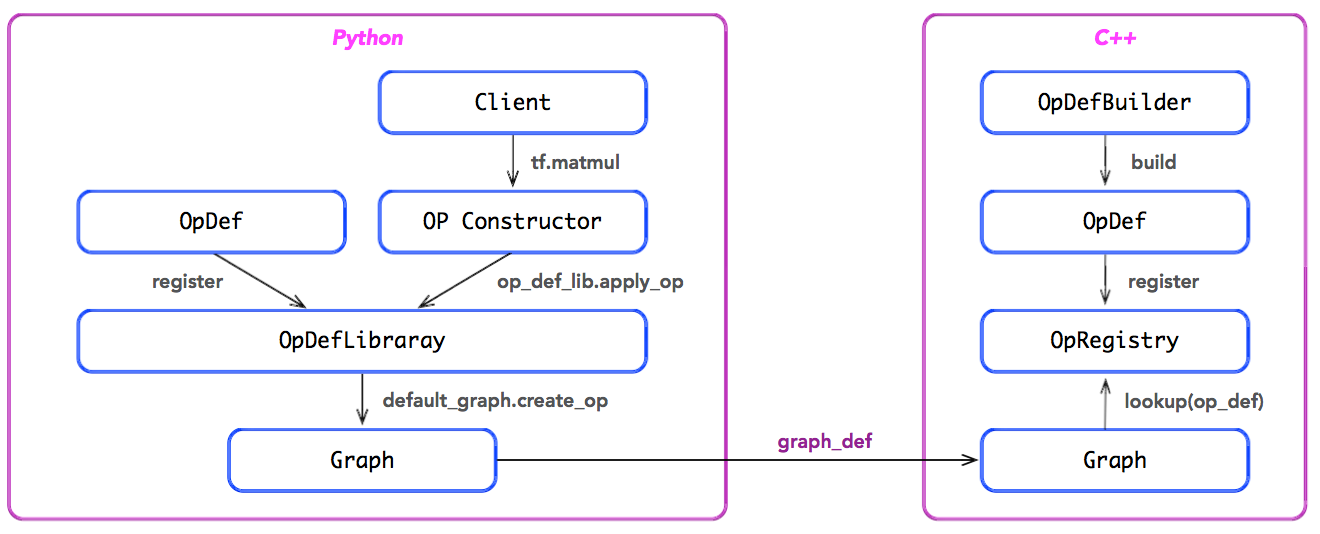
\includegraphics[width=0.9\textwidth]{figures/py-graph-creation.png}
\caption{图的序列化与反序列化}
 \label{fig:py-graph-creation}
\end{figure}

\end{content}

